\chapter{Frontend}
La segunda parte del sistema de auxilio es el cliente, \textbf{el código que se ejecuta en el dispositvo del usuario.}
\section{Elección de la tecnología}
Nunca hemos tenido tantas opciones:
\subsection{Web vs aplicación móvil}
Para el proyecto considero imprescindible que el cliente sea de la forma de \textbf{una aplicación móvil.} 
Una web app para este caso de uso la descarto por los siguientes motivos:
\begin{enumerate}
  \item Una app instalada es \textbf{más accesible} que entrar al navegador y después a una web.
  \item La cantidad de APIs a las que podemos acceder desde una aplicación es mayor. \textbf{Y necesito acceso a APIs muy concretas que no se pueden usar a traves del navegador.}
	\item \textbf{Ejecutar procedimientos en segundo plano en una web app cuando está cerrada no es posible.}
	\item \textbf{Recibir notificaciones push en iOS no es posible por medio de una web app.}
\end{enumerate}

\subsection{Framework de aplicación móvil}

\textbf{¿Qué características son deseables?}

\begin{enumerate}
  \item \textbf{Una base de código} para iOS y Android.
  \item \textbf{Paradigma declarativo}, que es más mantenible y claro que el imperativo.
  \item \textbf{Capacidad para utilizar funcionalidades nativas}, especificas del sistema operativo subyacente.
\end{enumerate}

\textbf{Por la primera característica, tengo que descartar Android e IOS nativo.} \\

\textbf{Plataformas que la cumplen: }
\begin{itemize}
  \item React Native \cite{reactnative}
  \item Nativescript \cite{nativescript}
  \item Ionic \cite{ionic}
  \item Quasar \cite{Quasar}
  \item Flutter \cite{flutter}
\end{itemize}

\textbf{Flutter vs React native}: Si bien es cierto que React Native tiene a favor la popularidad, un lenguaje al que ya estoy habituado y más estabilidad, es más lento que Flutter y hace una traducción de componentes a código nativo.
\textbf{Con Flutter sin embargo hay total control de los componentes y se muestran igual en las dos plataformas.} \\ \\

\textbf{Qasar e Ionic vs React native}: Qasar e Ionic son muy parecidos a React Native con menos popularidad, más posibilidad de frameworks como Vue o Angular pero usando 
una webview con acceso a APIs nativas via cordova. \\ \\

\textbf{Nativescript vs React Native:} Nativescript por último es similar a React Native, también en el método, ya que accede directamente a APIs nativas. \\ \\

\subsection{Lenguaje en la aplicación móvil}
\textbf{Flutter usa Dart} \cite{dart}, que es un lenguaje tipado que recuerda a Typescript: también con una hebra única y E/S no bloqueante.

\begin{figure}[H]
	\centering	
	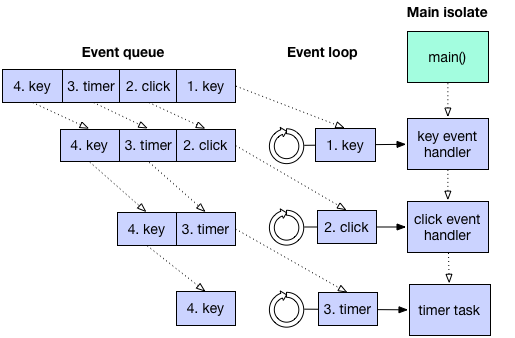
\includegraphics[scale=0.6]{dart.png}
	\caption{Funcionamiento del runtime de Dart}
	\end{figure}

\section{Diseño}
La parte de la solución que estamos implementando en este proyecto tiene unos inputs muy simples:
\begin{itemize}
	\item Activar alerta
	\item Desactivar alerta
	\item Escuchar alerta
	\item Cancelar escucha de alerta
\end{itemize}

\textbf{El FAB (floating action button)} que se situa abajo a la derecha realiza la primera, segunda y cuarta función. 
Cambia el icono central y su color dependiendo de la acción que dispara. En el caso de desactivar la alerta,
también se hace más grande para incluir un texto específico que podemos ver en la figura \ref{fig:alert}.

\begin{figure}[H]
	\centering	
	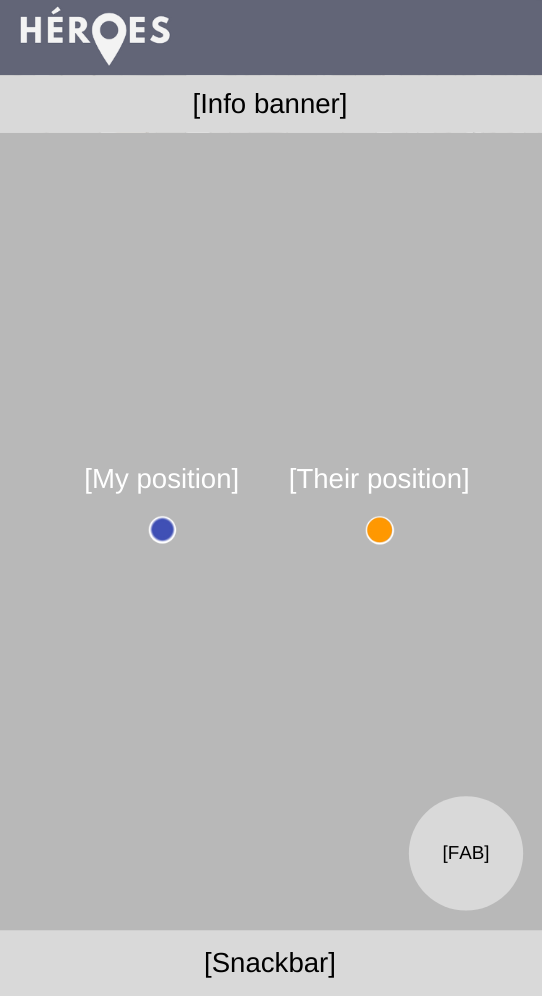
\includegraphics[scale=0.6]{mockup.png}
	\caption{Esquema de la aplicación}
	\end{figure}

Para escuchar una alerta, ha sido necesario incluir el \textbf{snackbar}, que emerge de la parte inferior de la aplicación cuando es necesario.
Esto es así, porque el usuario podría necesitar usar el FAB (en caso de necesitar ayuda) incluso si ha recibido una alerta. \\ \\

Por último, \textbf{para mostrar información tenemos el info banner y el mapa.} El primero informa al usuario una vez ha activado
una alerta de que esto se ha hecho con éxito, también informa de que se puede ver en el mapa la ubicación de la víctima en tiempo real
si está escuchando una alerta.

\section{Mapa}
En la aplicación, el mapa es muy protagonista. En él se ve representado el usuario y en caso de
atención a una alerta, también la víctima. \\ \\
Para implementarlo, \textbf{hay dos componentes:}
 \begin{itemize}
   \item \textbf{Provider de mapas:} Proporcionan los \textit{tiles} que no son más que imágenes que forman el mapa. \textbf{OpenStreetMap, por ejemplo}. Se puede configurar por variables de entorno en la aplicación.
   \item \textbf{Controlador:} Su función es \textbf{cargar y mostrar los \textit{tiles} en la pantalla}, además de \textbf{reaccionar a los gestos que hace el usuario} para moverse por el mapa. 
 \end{itemize}

 Estoy utilizando OpenStreetMap como provider \cite{openstreetmap} por ser uno de los pocos que se pueden utilizar gratuitamente. \\ \\
 Como controlador, Map Controller Library \cite{map}, porque es bastante maduro, customizable y compatible con cualquier provider.

\begin{figure}[H]
	\centering	
	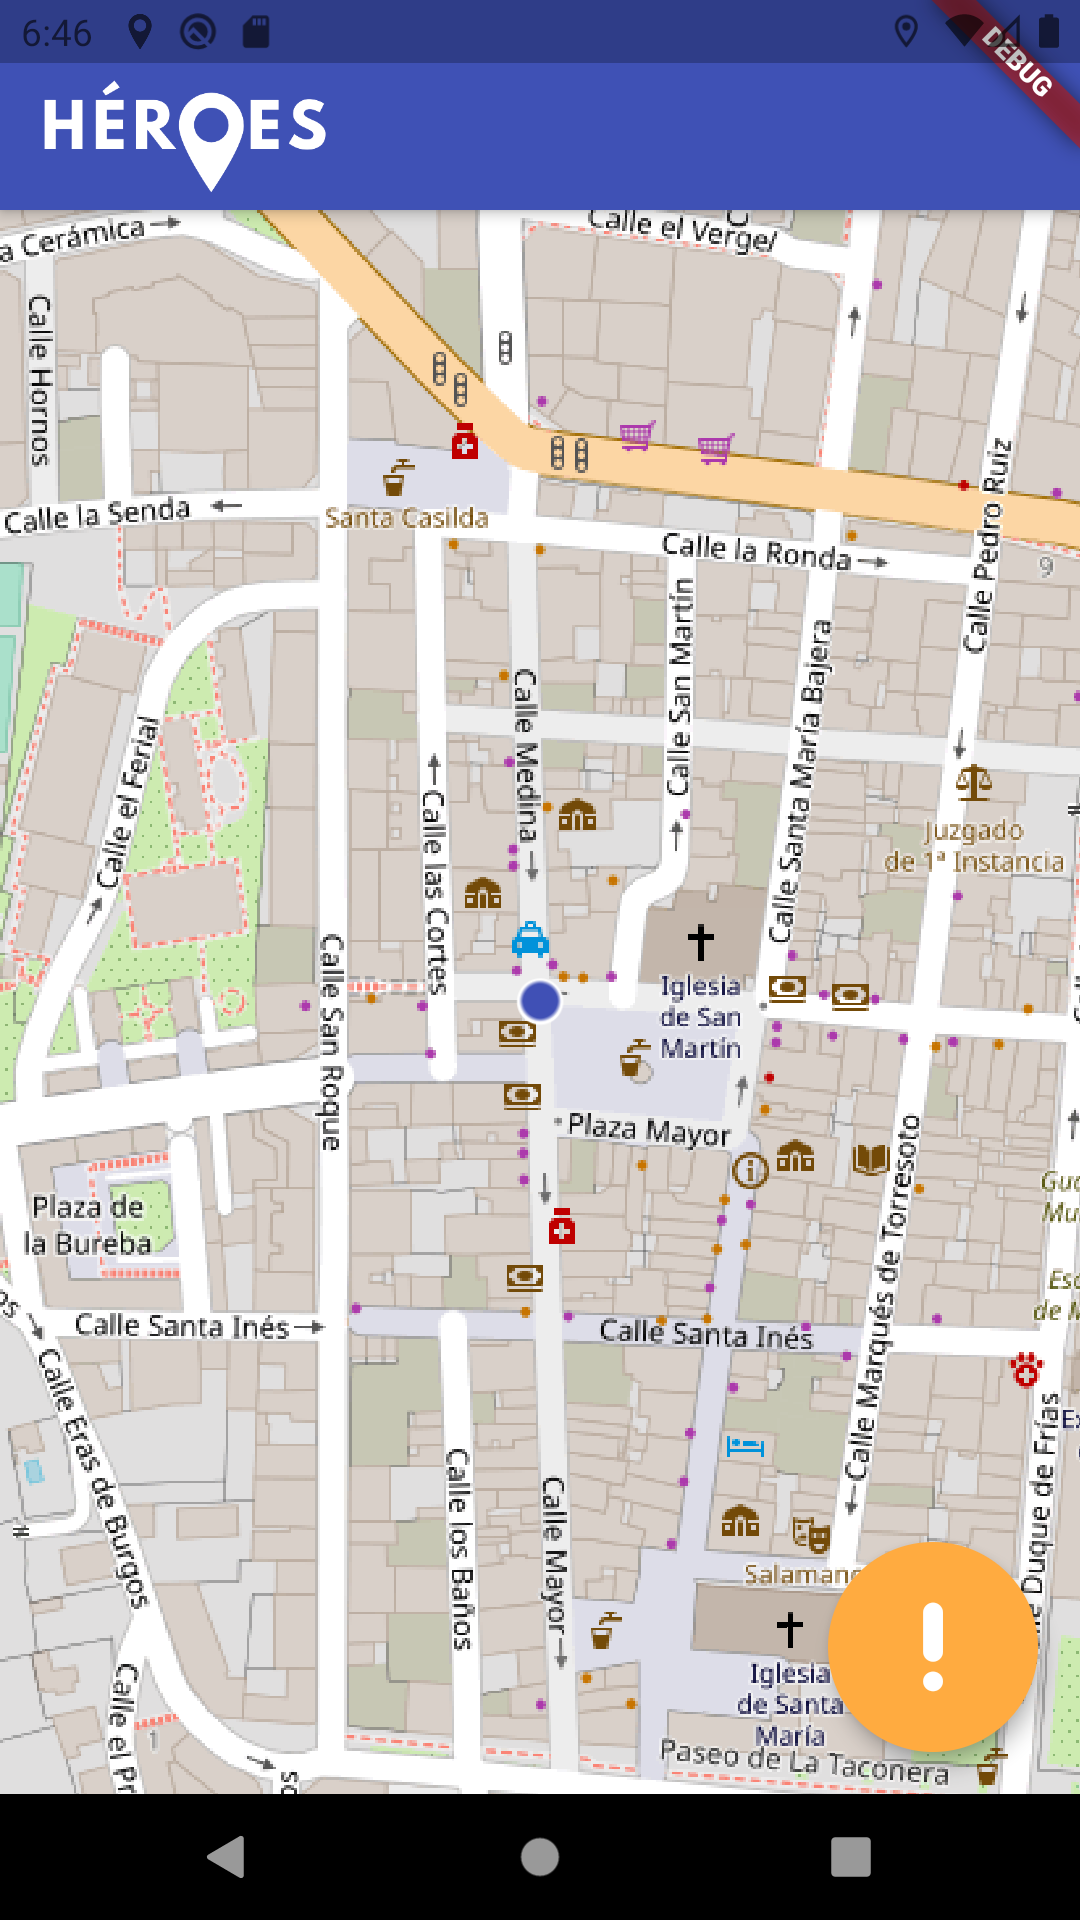
\includegraphics[scale=0.2]{home.png}
	\caption{Pantalla principal de la aplicación}
	\end{figure}

\section{Actualización de la localización}
Una parte fundamental de la aplicación es tener al día la ubicación del usuario para que \textbf{sea localizable en situación de alerta.} \\

En cualquiera de los siguientes escenarios:
\begin{itemize}
	\item La aplicación está en \textbf{primer plano.}
	\item La aplicación está \textbf{abierta en segundo plano.}
	\item La aplicación está \textbf{cerrada.}
\end{itemize}

Para ello, \textbf{he usado un isolate} (una hebra de Dart que se ejecuta aislada de la hebra principal, con un event loop independiente), que se comunica con la aplicación por medio de un Port (un canal entre hebras) y envía la ubicación actual al servidor. \\ \\
Además, usa APIs de Android que sacan partido a varios sensores del dispositivo para \textbf{disparar este 
proceso solo cuando el usuario realmente está en movimiento.}
También ha sido necesario registrar plugins como Firebase Cloud Messaging en java, para que estén disponibles en el isolate.

\section{Firebase Cloud Messaging}\label{sec:fib}
Como he anticipado en la sección \ref{sec:fibpre}, necesitamos un mecanismo para enviar notificaciones push a los usuarios en iOS y Android.
Además de integrar FCM en el servidor, también tenemos que hacerlo en el cliente para que las notificaciones lleguen en todos los escenarios.

\begin{itemize}
	\item La aplicación está en \textbf{primer plano.}
	\item La aplicación está \textbf{abierta en segundo plano.}
	\item La aplicación está \textbf{cerrada.}
\end{itemize}


Otra ventaja de usar FCM, es que nos permite obtener de manera sencilla un identificador único de dispositivo, que podemos usar en el servidor para enviar las notificaciones push.

\begin{figure}[H]
	\centering	
	
\includegraphics[scale=0.8]{notification.png}
	\caption{Notificación de alerta cuando la aplicación está cerrada}
	\end{figure}

\begin{figure}[H]
	\centering	
	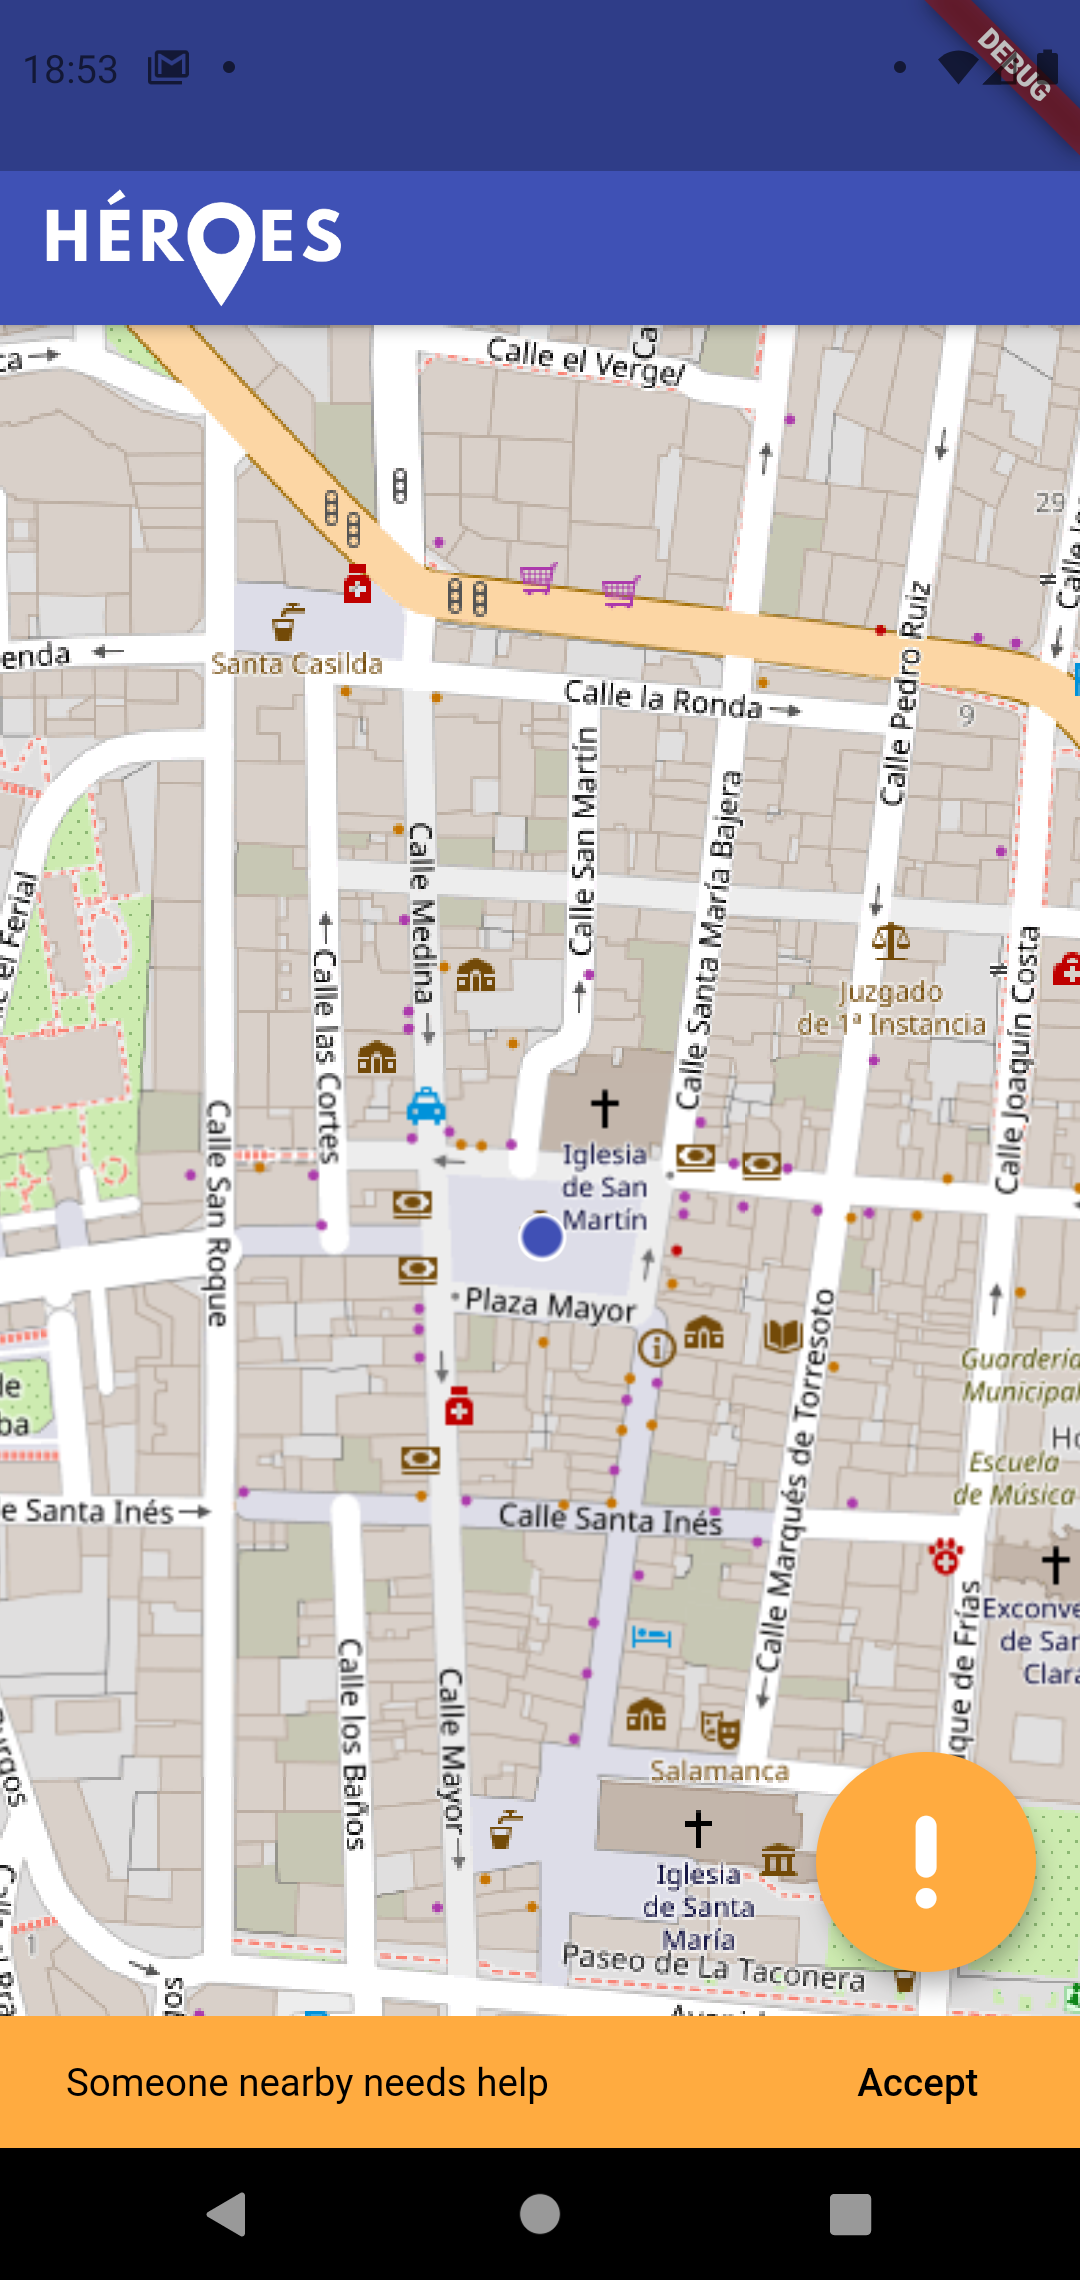
\includegraphics[scale=0.2]{notification-inapp.png}
	\caption{Notificación de alerta cuando la aplicación está abierta}
	\end{figure}

\section{Websockets}

Para obtener actualizaciones respecto a una alerta una vez la estamos escuchando, utilizamos el endpoint del que hemos hablado en \ref{subsec:websocket} mediante websockets.
He usado una librería \cite{websocketchannel} para esto.

\begin{figure}[H]
	\centering	
	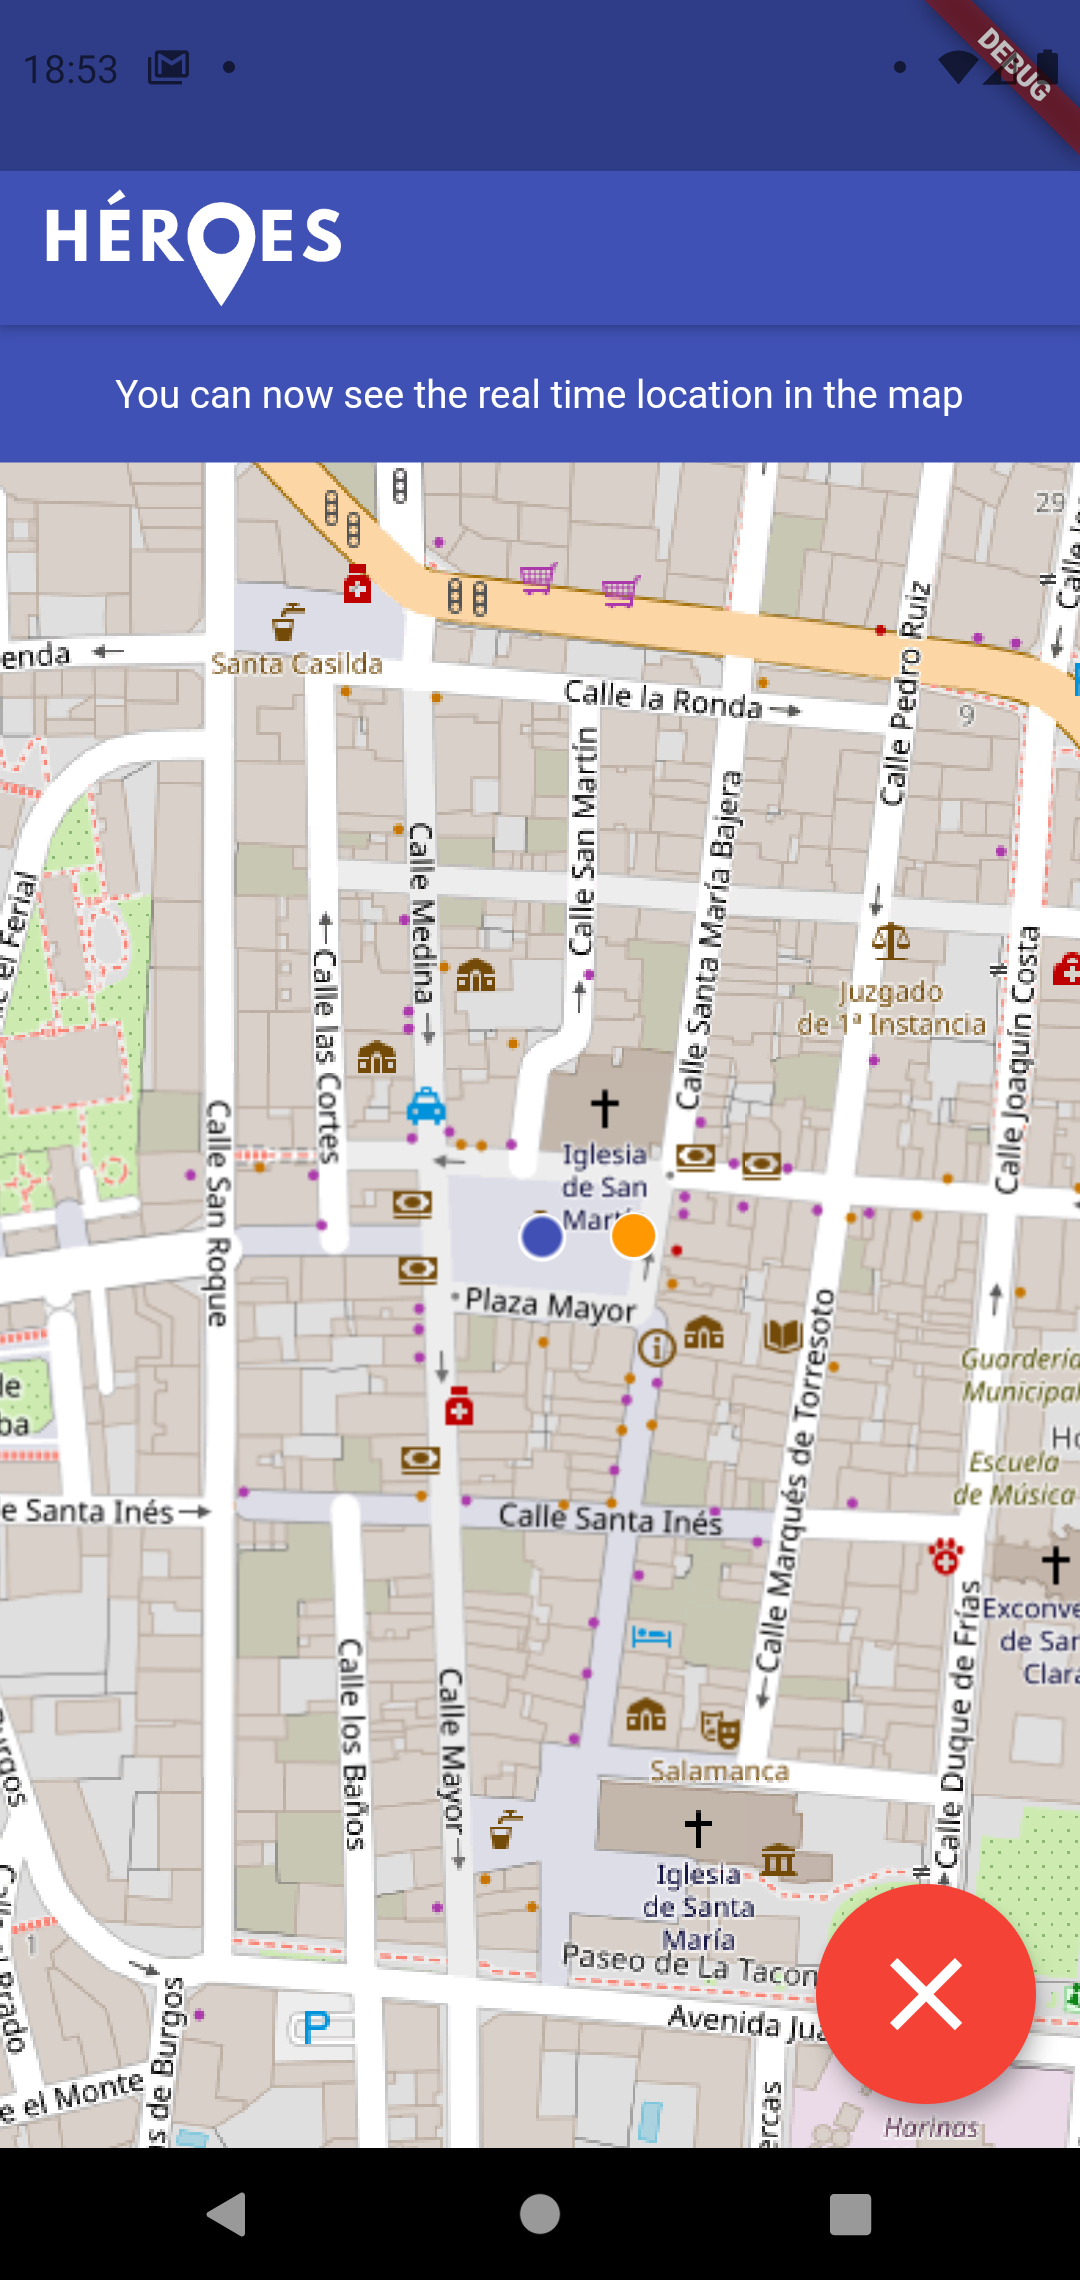
\includegraphics[scale=0.2]{watch-alert.png}
	\caption{Pantalla de seguimiento de alerta, actualización de la ubicación de la víctima y del estado de la alerta en tiempo real}
	\end{figure}

\section{Manejo del estado}
\textbf{En flutter}, como en otros frameworks (React, Vue, Angular, etc...), \textbf{se crea un árbol de componentes.}
Los datos fluyen de arriba a abajo, de padres que saben más a hijos que saben
menos. Y los eventos de abajo a arriba, \textbf{los hijos informan a los padres de cambios mediante callbacks.}
\begin{figure}[H]
	\centering	
	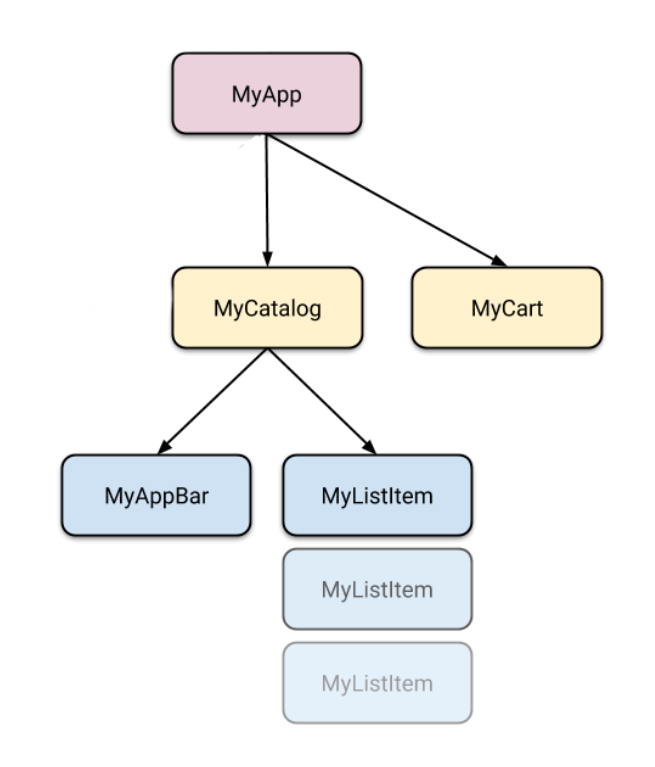
\includegraphics[scale=0.3]{tree.png}
	\caption{Un árbol de componentes}
	\end{figure}
Sin embargo, hay veces que \textbf{ciertos datos o comportamientos deben ser
expuestos para muchos componentes.} También puede pasar que no se necesiten
en componentes superficiales y sean necesarios en otros muy profundos. \\ \\
En un ecosistema tan grande como el de Flutter, tenemos varias propuestas, más y
menos sofisticadas. Redux, BLoC/Rx o MobX son algunos ejemplos, adecuadas
para casos más pesados.\\ \\
En mi opinión, \textbf{para aplicaciones pequeñas/medianas Provider es un \textit{sweet spot}
entre no usar estado de aplicación y usar uno muy potente.} \\ \\

Para esta aplicación, tiene mucho sentido porque los datos no tienen estructura jerárquica, como, digamos, un e-commerce. \\
He utilizado dos providers que \textbf{exponen comportamiento y datos muy cohesionados:}
\begin{itemize}
	\item \textbf{Geolocalization provider:} Que ofrece getters y setters sobre el servicio de actualización en segundo plano y la localización actual.
	\item \textbf{Alert provider:} Que crea y realiza el seguimiento de alertas. También mantiene el estado sobre el rol del usuario (emitiendo alerta, standby, escuchando alerta, etc...).
\end{itemize}

\begin{figure}[H]\label{fig:alert}
	\centering	
	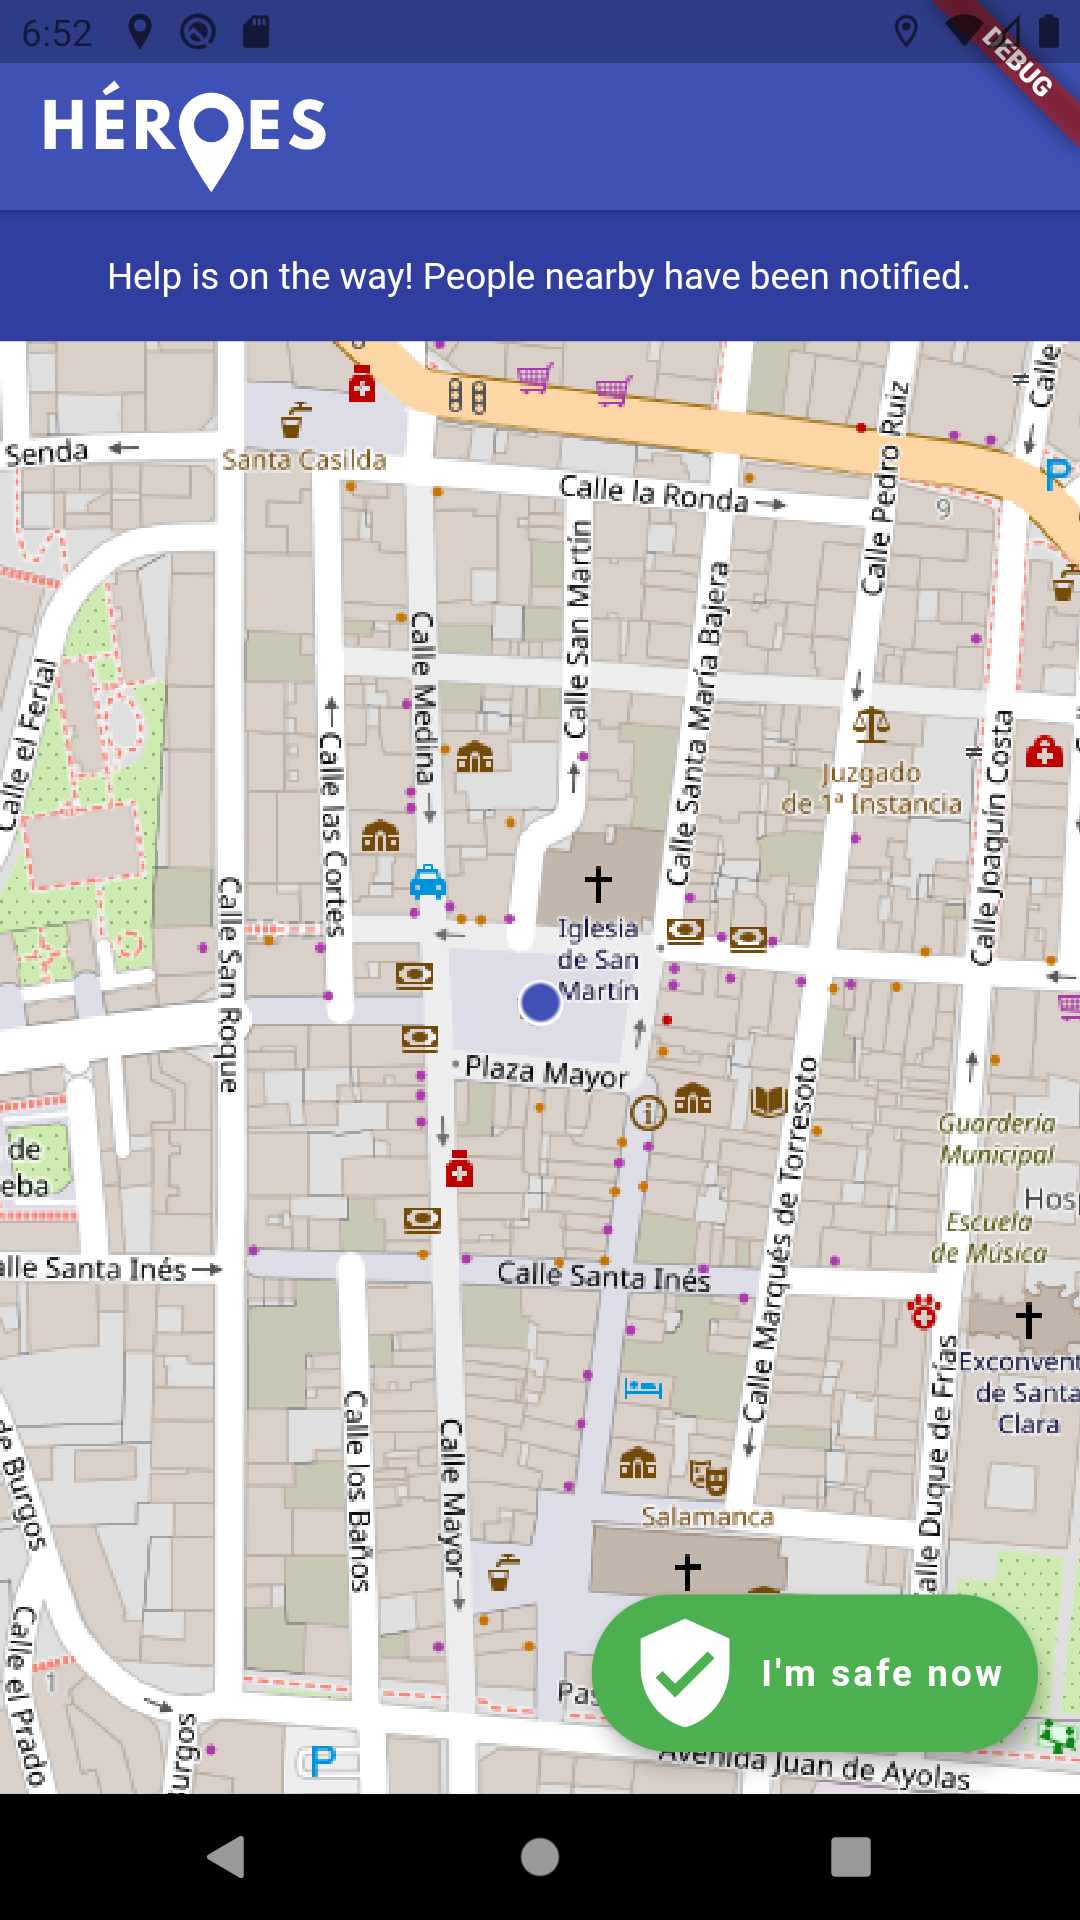
\includegraphics[scale=0.2]{create-alert.png}
	\caption{La aplicación después de crear una alerta. Los componentes reaccionan a cambios en los providers.}
	\end{figure}

